\documentclass{article}

\usepackage{calculator}
\usepackage{calculus}

\usepackage{fancyhdr}
\usepackage{extramarks}
\usepackage{amsmath}
\usepackage{amsthm}
\usepackage{amsfonts}
\usepackage{tikz}
\usepackage[plain]{algorithm}
\usepackage{algpseudocode}
\usepackage{tikz,pgfplots,multicol}
\usepackage[font=small,labelformat=empty]{caption}
\usetikzlibrary{automata,positioning,arrows,patterns}
\usepackage{enumitem}

%
% Basic Document Settings
%

\topmargin=-0.45in
\evensidemargin=0in
\oddsidemargin=0in
\textwidth=6.5in
\textheight=9.0in
\headsep=0.25in

\linespread{1.1}

\pagestyle{fancy}
\lhead{\hmwkAuthorName}
\chead{\hmwkClass\ (\hmwkClassInstructor\ \hmwkClassTime)}
\rhead{\hmwkTitle}
\lfoot{\lastxmark}
\cfoot{\thepage}

\renewcommand\headrulewidth{0.4pt}
\renewcommand\footrulewidth{0.4pt}

\setlength\parindent{0pt}

\setcounter{secnumdepth}{0}
\newcounter{partCounter}
\newcounter{homeworkProblemCounter}
\setcounter{homeworkProblemCounter}{1}
\nobreak\extramarks{Problem \arabic{homeworkProblemCounter}}{}\nobreak{}

%
% Homework Problem Environment
%
% This environment takes an optional argument. When given, it will adjust the
% problem counter. This is useful for when the problems given for your
% assignment aren't sequential. See the last 3 problems of this template for an
% example.
%
\newenvironment{homeworkProblem}[1][-1]{
    \ifnum#1>0
        \setcounter{homeworkProblemCounter}{#1}
    \fi
    \section{Problem \arabic{homeworkProblemCounter}}
    \setcounter{partCounter}{1}
    \enterProblemHeader{homeworkProblemCounter}
}{
    \exitProblemHeader{homeworkProblemCounter}
}

%
% Homework Details
%   - Title
%   - Due date
%   - Class
%   - Section/Time
%   - Instructor
%   - Author
%

\newcommand{\hmwkTitle}{HW \#9}
\newcommand{\hmwkDueDate}{March 16, 2017}
\newcommand{\hmwkClass}{MATH 1300}
\newcommand{\hmwkClassTime}{Section 005}
\newcommand{\hmwkClassInstructor}{Professor Braden Balentine}
\newcommand{\hmwkAuthorName}{\textbf{John Keller}}

%
% Title Page
%

\title{
    \vspace{2in}
    \textmd{\textbf{\hmwkClass:\ \hmwkTitle}}\\
    \normalsize\vspace{0.1in}\small{Due\ on\ \hmwkDueDate\ at 10:00am}\\
    \vspace{0.1in}\large{\textit{\hmwkClassInstructor\ \hmwkClassTime}}
    \vspace{3in}
}

\author{\hmwkAuthorName}
\date{}

\renewcommand{\part}[1]{\textbf{\large Part \Alph{partCounter}}\stepcounter{partCounter}\\}

%
% Various Helper Commands
%

% Useful for algorithms
\newcommand{\alg}[1]{\textsc{\bfseries \footnotesize #1}}

% For derivatives
\newcommand{\deriv}[1]{\frac{\mathrm{d}}{\mathrm{d}x} (#1)}

% For partial derivatives
\newcommand{\pderiv}[2]{\frac{\partial}{\partial #1} (#2)}

% Integral dx
\newcommand{\dx}{\mathrm{d}x}

% Alias for the Solution section header
\newcommand{\solution}{\textbf{\large Solution}}

% Probability commands: Expectation, Variance, Covariance, Bias
\newcommand{\E}{\mathrm{E}}
\newcommand{\Var}{\mathrm{Var}}
\newcommand{\Cov}{\mathrm{Cov}}
\newcommand{\Bias}{\mathrm{Bias}}


\usepackage{xcolor}
    \colorlet{Curve}{red!75!black}
    \colorlet{Tangent}{blue!75!black}
\usepackage{pgfplots}
    \pgfplotsset{compat=1.10}
    \usetikzlibrary{
        calc,
        intersections,
        math,
    }
    \makeatletter
        \def\parsenode[#1]#2\pgf@nil{%
            \tikzset{label node/.style={#1}}
            \def\nodetext{#2}
        }
        \tikzset{
            % define style for the points
            Point/.style={
                shape=circle,
                inner sep=0pt,
                minimum size=3pt,
            },
            add node at x/.style 2 args={
                name path global=plot line,
                /pgfplots/execute at end plot visualization/.append={
                        \begingroup
                        \@ifnextchar[{\parsenode}{\parsenode[]}#2\pgf@nil
                    \path [name path global = position line #1-1]
                        ({axis cs:#1,0}|-{rel axis cs:0,0}) --
                        ({axis cs:#1,0}|-{rel axis cs:0,1});
                    \path [xshift=1pt, name path global = position line #1-2]
                        ({axis cs:#1,0}|-{rel axis cs:0,0}) --
                        ({axis cs:#1,0}|-{rel axis cs:0,1});
                    \path [
                        name intersections={
                            of={plot line and position line #1-1},
                            name=left intersection
                        },
                        name intersections={
                            of={plot line and position line #1-2},
                            name=right intersection
                        },
                        label node/.append style={pos=1}
                    ] (left intersection-1) -- (right intersection-1)
                        node [label node]{\nodetext};
                    % ---------------------------------------------------------
                    % draw the tangent line from a bit right of the point on
                    % the curve to the intersection with the ordinate
                    % and draw the corresponding points
                    \draw [dashed] let
                        \p1=($ (left intersection-1) - (right intersection-1) $),
                        \p2=($ (left intersection-1)!sign(#1)*10mm!(right intersection-1) $),
                        %\p2=($ (left intersection+1) - (right intersection+1) $),
                        \p3=($ ({axis cs:0,0}) - (\p2) $),
                        \n1={\x3/\x1}	% slope of tangent line
                    in
                        (\p2) -- +($ {\n1}*(\x1,\y1) $)
	                        
%                        		node[right,node font=\scriptsize,gray] {$y=$\y1/\x1*sign(#1) $x+$}
%                            node [Point,fill=Tangent] (origin intersection) {}
                            node [Point,fill=Curve] at (left intersection-1) {}
                    ;
                    % ----------
                    % draw the horizontal line at the curve intersection point
                    % plus the label above/below the line
%                    \tikzmath{
%                        coordinate \c1;
%                        \c1=(left intersection-1) - (right intersection-1);
%                        \slope=\cy1/\cx1*sign(#1);
%                        \plusoffset = (#1+1);
%                    }
%                    \pgfmathsetmacro{\AboveBelow}{ \slope>0 ? "above" : "below" }
%                    \draw [dashed]
%                        ([xshift=sign(#1)*2.5mm] left intersection-1) --
%                        (left intersection-1) --
%                            node [\AboveBelow,node font=\scriptsize] {$y=\slope x+\plusoffset$}
%                        (left intersection-1 -| origin intersection) --
%                        +($ sign(#1)*(-2.5mm,0) $)
%                            coordinate [pos=0.5] (a)
%                    ;
%                    % draw the horizontal line at the ordinate intersection point
%                    \draw [dotted] (origin intersection)
%                        +($ sign(#1)*(-2.5mm,0) $) --
%                        (origin intersection);
%                    % draw vertical line left/right of the ordinate
%                    \pgfmathsetmacro{\LeftRight}{ #1<0 ? "right" : "left" }
%                    \draw [stealth-stealth] (origin intersection)
%                        +($ sign(#1)*(-1.25mm,0) $) -- (a)
%                            node [midway,\LeftRight,node font=\scriptsize] {$p$}
%                    ;
%                    % ---------------------------------------------------------
                        \endgroup
                },
            },
        }
    \makeatother
\makeatletter
\def\mathcolor#1#{\@mathcolor{#1}}
\def\@mathcolor#1#2#3{%
  \protect\leavevmode
  \begingroup
    \color#1{#2}#3%
  \endgroup
}
\makeatother


\begin{document}

\maketitle

\pagebreak

\section{Section 3.7}

\begin{enumerate}
\setcounter{enumi}{28}
	\item
		\begin{enumerate}
			\item On what interval is $f(x)=x\ln x$ decreasing?
			$$\begin{align}
				f'(x)&=\ln(x)\Big(\frac{d}{dx}(x)\Big)+x\Big(\frac{d}{dx}\big(\ln(x)\big)\Big)\\
				&=x\Big(\frac{d}{dx}\big(\ln(x)\big)\Big)+\ln(x)\\
				&=\ln(x)+\frac{1}{x}x\\
				&=1+\ln(x)
			\end{align}$$
			\vspace{1cm}
			\item On what interval is $f$ concave upward?
			$$\begin{align}
				f''(x)&=\frac{d}{dx}\big(1+\ln(x)\big) \\
				&=\frac{d}{dx}\big(\ln(x)\big)\\
				&=\frac{1}{x}
			\end{align}$$
			\vspace{1cm}
		\end{enumerate}
\setcounter{enumi}{31}
	\item Let $f(x)=\log_a(3x^2-2)$. For what value of $a$ is $f'(1)=3$?	
	$$\begin{align}
		f'(x)&=\frac{d}{dx}\big(\log_a(3x^2-2)\big)\\
		&=\frac{d}{dx}\Big(\frac{\log(3x^2-2)}{\log(a)}\Big) \\
		&=\frac{\frac{d}{dx}(3x^2-2)}{(3x^2-2)\log(a)}\\
		&=\frac{3(\frac{d}{dx}(x^2))}{(3x^2-2)\log(a)}\\
		&=2x\frac{3}{(3x^2-2)\log(a)}\\
		3&=\frac{6x}{(3x^2-2)\log(a)}\\
		3(3x^2-2)\log(a)&=6x\\
		9x^2-6\cdot3\log(a)&=6x\\
		3\log(a)&=6x-9x^2+6\\
		\log(a)&=2(1)-3(1)^2+2\\
		\log(a)&=1\\
		10^a&=1\\
		a&=e
	\end{align}$$
\setcounter{enumi}{33}
	\item Use logarithmic differentiation to find the derivative of the function $y=\sqrt{x}e^x^2(x^2+1)^{10}$.
	$$\begin{align}
		\frac{d}{dx}(y)&=\frac{d}{dx}(\sqrt{x}e^x^2(x^2+1)^{10})\\
		&=\sqrt{x}(1+x^2)^{10}(\frac{d}{dx}(e^{x^2})+e^{x^2}(\frac{d}{dx}(\sqrt{x}(1+x^2)^{10} ))\\
		&=e^{x^2}(\frac{d}{dx}(\sqrt{x}(1+x^2)^{10})+e^{x^2}\frac{d}{dx}(x^2)\sqrt{x}(1+x^2)^{10}\\
		&=2e^{x^2}x^{\frac{3}{2}}(1+x^2)^{10}+e^{e^2}(\frac{d}{dx}(1+x^2)^{10})\\
		&=2e^{x^2}x^{\frac{3}{2}}(1+x^2)^{10}+e^{x^2}(\frac{(1+x^2)^{10}}{2\sqrt{x}}+2x10\sqrt{x}(1+x^2)^9)\\
		&=\boxed{2e^{x^2}x^{\frac{3}{2}}(1+x^2)^{10}+e^{x^2}(20x^{\frac{2}{3}}(1+x^2)^9+\frac{(1+x^2)^{10}}{2\sqrt{x}}}
	\end{align}$$
\setcounter{enumi}{37}
	\item Use logarithmic differentiation to find the derivative of the function $y=x^{\cos x}$.
	$$\begin{align}
		y&=x^{\cos x}\\
		\ln y &= \cos x \ln x\\
		\frac{1}{y}dy &= (-\sin x \ln x + \frac{\cos x}{x} )dx\\
		\frac{dy}{dx} &= (y)(-\sin x \ln x + \frac{\cos x}{x} )\\
		\frac{dy}{dx} &= \boxed{x^{\cos x} (-\sin x \ln x + \frac{\cos x}{x} )}
	\end{align}$$
\setcounter{enumi}{44}
	\item Find a formula for $(f^{(n)})(x)$ if $f(x)=\ln(x-1)$.
	$$\begin{align}
		\frac{d}{dx}f^{(n)}(x)&=\frac{d}{dx}\left( \frac{(-1)^{n-1}(n-1)}{(x-1)^n}\right) \\
		&= (-1)^{n-1}(n-1)\frac{d}{dx}\left((x-1)^{-n}\right) \\
		&= (-1)^{n-1}(n-1)\left( (-n)(x-1)^{-n-1}\right) \\
		&= \boxed{\frac{(-1)^{n}n}{(x-1)^{n+1}}} \\
	\end{align}$$
\end{enumerate}

\section{Section 3.8}
\begin{enumerate}
\setcounter{enumi}{5}
	\item Graphs of the \textit{position} functions of two particles are shown, where $t$ is measured in seconds. When is each particle speeding up? When is it slowing down? Explain.
	\begin{center}
		\begin{minipage}{0.05\linewidth}\vspace{0pt}
		(a)	
		\end{minipage}
		\begin{minipage}{0.4\linewidth}
			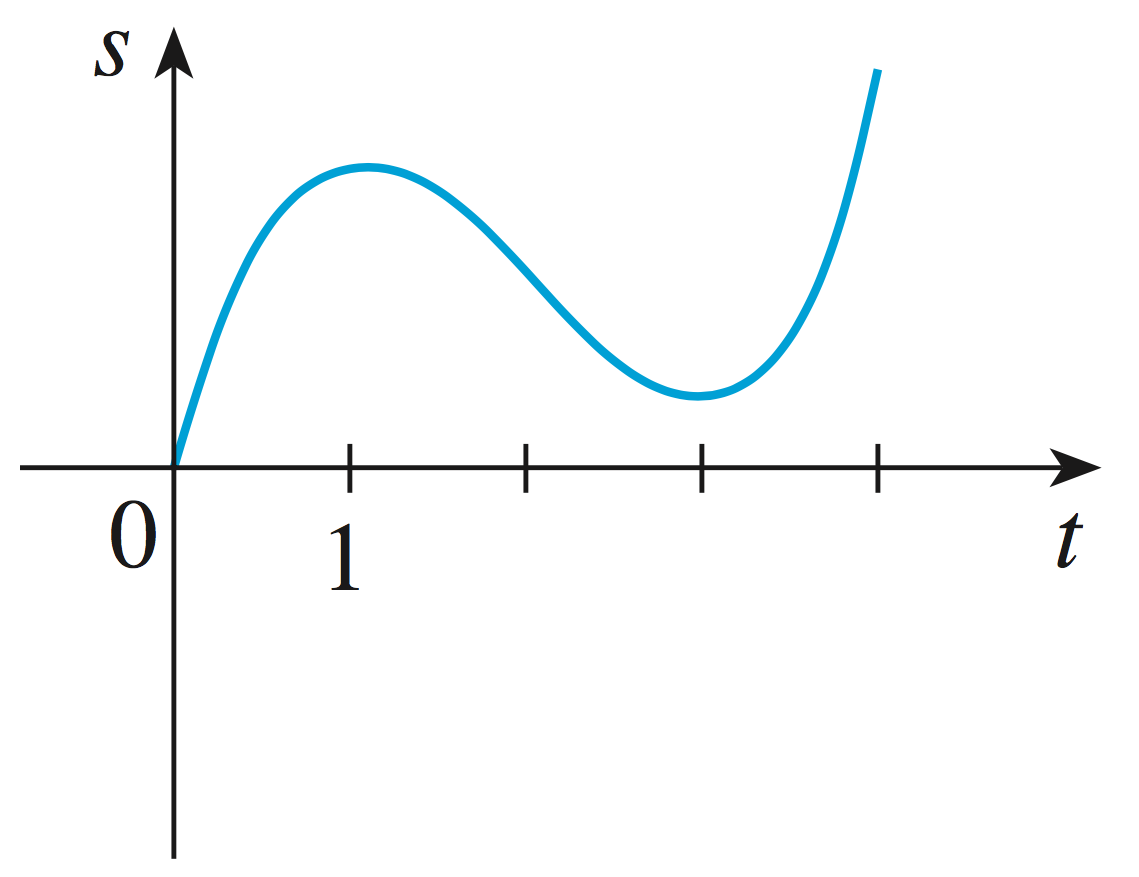
\includegraphics[width=4cm]{images/37pr6a.png}\newline
			The cup is speeding up at $(0,1)\cup(3,4)$ because $t'(s)$ is positive, and slowing down at $(1,3)$ because the tangent is negative.
		\end{minipage}
		\begin{minipage}{0.05\linewidth}
		(b)	
		\end{minipage}
		\begin{minipage}{0.4\linewidth}
			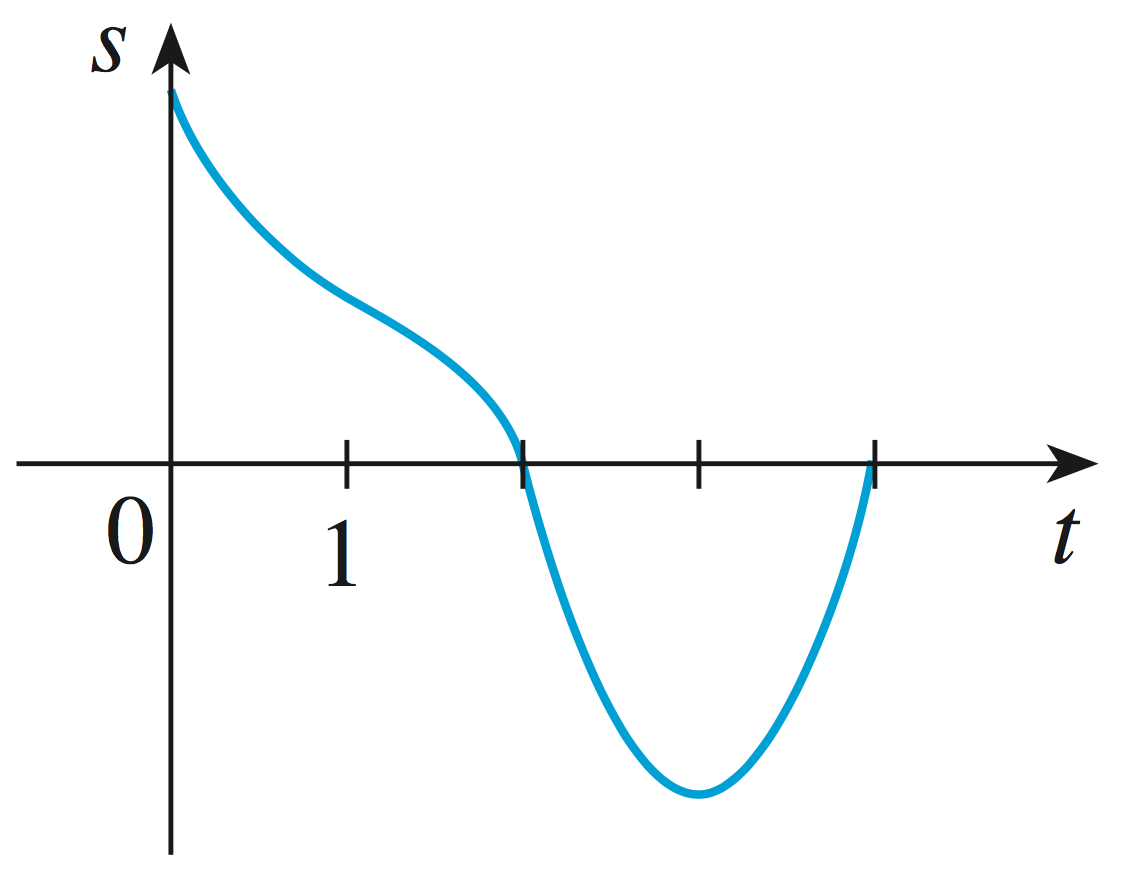
\includegraphics[width=4cm]{images/37pr6b.png}\newline
			The cup is speeding up at $(3,4)$ because $t'(s)$ is positive, and slowing down at $(0,3)$ because the tangent is negative.
		\end{minipage}
	\end{center}
\setcounter{enumi}{9}
	\item If a ball is thrown vertically upward with a velocity of 80 ft/s, then its height after $t$ seconds is $s=80t-16t^2$.
		\begin{enumerate}
			\item What is the maximum height reached by the ball?
			$$\begin{align}
				s'(t)&=80-32t\\
				0&=80-32t\\
				-80&=-32t\\
				t&=\frac{5}{2}\\
				s&=80\Big(\frac{5}{2}\Big)-16\Big(\frac{5}{2}\Big)^2\\
				&=200-16\Big(\frac{25}{4}\Big)\\
				&=200-100\\
				&=\boxed{100\text{ ft.}}
			\end{align}$$
			\item What is the velocity of the ball when it is 96 ft above the ground on its way up? On its way down?
				$$\begin{align}
					96&=80t-16t^2\\
					t&=2 \text{ or } 3\\
					s'(2)&=80-32(2)\\
					s'(2)&=16\\
					s'(3)&=80-32(3)\\
					s'(3)&=-16
				\end{align}$$
				On the way up, the velocity is 16 ft/min, on the way down the velocity is -16 ft/min.
		\end{enumerate}
\setcounter{enumi}{23}
	\item The number of yeast cells in a laboratory culture increases rapidly initially but levels off eventually. The population is modeled by the function $$n=f(t)=\frac{a}{1+be^{-0.7t}}$$ where $t$ is measured in hours. At time $t=0$ the population is 20 cells and is increasing at a rate of 12 cells/hour. Find the values of $a$ and $b$. According to this model, what happens to the yeast population in the long run?
	$$\begin{align}
		f'(t)&=\frac{0.7abe^{-0.7t}}{(1+be^{-0.7t})^2}\\
		f'(0)&=12\\
		12&=\frac{0.7ab}{(1+b)^2}\\
		0.7ab&=12(1+b)^2\\
		a&=140\\
		b&=6\\
		\underset{t\rightarrow\infty}{\text{lim}}f(t)&=\frac{a}{1+b}\underset{t\rightarrow\infty}{\text{lim}}e^{-0.7t}\\
		\underset{t\rightarrow\infty}{\text{lim}}f(t)&=\frac{a}{1+b\cdot 0}\\
		\underset{t\rightarrow\infty}{\text{lim}}f(t)&=\frac{a}{1}\\
		\underset{t\rightarrow\infty}{\text{lim}}f(t)&=a
	\end{align}$$
	According to the model, as time goes on, the number of cells will get infinitely closer to 140, but never actually reach 140.
\setcounter{enumi}{29}
	\item The cost function for production of a commodity is $$C(x)=339+25x-0.09x^2+0.0004x^3$$
	\begin{enumerate}
		\item Find and interpret $C'(200)$.
		$$\begin{align}
			C'(x)&=25-0.18x+0.0012x^2\\
			C'(200)&=25-0.18(200)+0.0012(200)^2\\
			C'(200)&=37
		\end{align}$$
		The number 37 tells us that the cost for the production of a commodity is is increasing at \$37/item. This means producing one more item (for a total of 201) would cost \$37.
		\item Compare $C'(100)$ with the cost of producing the 101st item.
		$$\begin{align}
			C'(100)&=25-0.18(100)+0.0012(100)^2\\
			C'(100)&=19\\
			C(101)&=339+25(101)-0.09(101)^2+0.0004(101)^3\\
			C(101)&=\$2358.0304
		\end{align}$$
		This means that using $C'(x)$, you can estimate that the cost of producing the 100th item as $2358.0304-19=2339.034$.
	\end{enumerate}
\end{enumerate}
\pagebreak
\section{Section 3.9}
\begin{enumerate}
\setcounter{enumi}{5}
	\item The table shows the population of Nepal (in millions) as of June 30th of the given year. Use linear approximation to estimate the population at midyear in 1989. Use another linear approximation to predict the population in 2010.
	\begin{center}
		\begin{tabular}{|l|l|l|l|l|l|}\hline
		$t$    & 1985  & 1990  & 1995  & 2000  & 2005  \\ \hline
		$N(t)$ & 17.04 & 19.33 & 21.91 & 24.70 & 27.68 \\ \hline
		\end{tabular}
	\end{center}
	$$\begin{align}
		L(t)&=N(1990)+N'(1990)(t-1990)\\
		&=19.33+N'(1990)(t-1990)\\
		N'(1990)&\approx\frac{1}{2}\Bigg(\Big(\frac{21.91-19.33}{1995-1990} \Big)+\Big(\frac{19.33-17.04}{1990-1985} \Big)\Bigg)\\
		N'(1990)&\approx \frac{1}{2}(0.5160+0.4580)\\
		N'(1990)&\approx 0.4870\\
		L(t)&=19.33+0.4870(t-1990)\\
		L(1989.5)&\approx 19.33+0.4870(1989.5-1990)\\
		L(1989.5)&\approx \boxed{19.1 \text{ million people}}\\ \hline
		L(t)&=N(2005)+N'(2005)(t-2005)\\
		&=27.68+N'(2005)(t-2005)\\
		N'(2005)&\approx\Big(\frac{27.68-24.70}{2005-2000} \Big)\\
		N'(2005)&\approx 0.596\\
		L(t)&=27.68+0.596(t-2005)\\
		L(2010)&=27.68+0.596(2010-2005)\\
		L(2010)&=\boxed{30.66 \text{ million people}}
	\end{align}$$
\setcounter{enumi}{9}
	\item Find the linear approximation of the function $g(x)=\sqrt[\leftroot{-2}\uproot{2}3]{1+x}$ at $a=0$ and use it to approximate the numbers $\sqrt[\leftroot{-2}\uproot{2}3]{0.95}$ and $\sqrt[\leftroot{-2}\uproot{2}3]{1.1}$. Illustrate by graphing $g$ and the tangent line.
	$$\begin{align}
		f'(x)&=\frac{1}{3\sqrt[\leftroot{-2}\uproot{2}3]{(1+x)^2}}\\
		L(x)&=f(0)+f'(0)(x-0)\\
		L(x)&=1+\frac{x}{3}\\
		L(\sqrt[\leftroot{-2}\uproot{2}3]{0.95})\approx 1+\frac{-0.05}{3}\approx 0.9833\\
		L(\sqrt[\leftroot{-2}\uproot{2}3]{1.1})\approx 1+\frac{0.1}{3}\approx 1.0333
	\end{align}$$
	\begin{center}
		\pgfplotsset{width=13cm,height=8cm, axis equal}
			\begin{tikzpicture}
			\begin{axis}[axis lines=middle,minor y tick num=0,minor x tick num=0,tick style={black},grid style={solid, gray!20}]
				\addplot[domain=-5:5, samples=100] {(1+x)/abs((1+x))*abs((1+x))^(1/3)};
				\addplot[domain=-5:5,dashed] {1+(x/3)};
			\end{axis}
		\end{tikzpicture}
	\end{center}
\setcounter{enumi}{19}
	\item Explain, in terms of linear approximation or differentials, why the approximation is reasonable for $(1.01)^6\approx 1.06$.
	$$\begin{align}
		L(x)&=f(a)+f'(a)(x-a)\\
		&=f(1)+f'(1)(x-1)\\
		&=1^6+6(1)^5(x-1)\\
		&=1+6(x-1)\\
		L(1.01)&=1+6(1.01-1)\\
		&=1+6(0.01)\\
		&=\boxed{1.06}
	\end{align}$$
\setcounter{enumi}{29}
	\item Use differentials to estimate the amount of paint needed to apply a coat of paint 0.05 cm thick to a hemispherical dome with diameter 50 m.
	$$\begin{align}
		V&=\frac{2}{3}\pi r^3\\
		dV&=\frac{2}{3}3\pi r^2dr\\
		dV&=2\pi r^2 dr\\
		dV&=2\pi(25)^2(0.05)\\
		dV&=\boxed{\frac{125\pi}{2}\text{ cm}^3}
	\end{align}$$
\end{enumerate}

%
\end{document}